% !TEX program = xelatex
\documentclass[10pt,aspectratio=169]{beamer}
\usetheme{default}
\setbeamertemplate{navigation symbols}{}
\setbeamerfont{frametitle}{size=\large,series=\bfseries}
\setbeamercolor{frametitle}{fg=white,bg=green!50!black}
\setbeamercolor{title}{fg=green!50!black}
\setbeamercolor{structure}{fg=green!40!black}
\setbeamertemplate{frametitle}[default][shadow=false]
\addtobeamertemplate{frametitle}{\vspace{2pt}}{\vspace{2pt}}
\usepackage{xeCJK}
\setCJKmainfont{Noto Serif TC}
\usepackage{amsmath,amssymb}
\usepackage{booktabs}
\usepackage{graphicx}
\usepackage{tikz}

\title{便利商店最佳化餐食推薦}
\subtitle{以 MILP + GRASP-LS 啟發式並用之最佳化決策架構}
\author{Group 13: B13705005 宋宇倫、B13705011 陳芃慈、B13705020 陳鼎元、B13705029 蔡冠毅}
\institute{Department of Information Management, NTU}
\date{Operations Research 2026, Final Project}

\begin{document}

\maketitle

% ============================================================
\section{Motivation}
\begin{frame}{背景與動機}
\textbf{便利商店} 已是大學生與上班族最高頻次的即時餐食管道：
\begin{itemize}
  \item 門市密度高、購買快速、商品標示完整
  \item 但同時面對：成本、熱量、蛋白質、糖、鈉、飽足感等多重考量
  \item 還有「飯糰＋飲料」、「麵食＋蛋」等捆綁優惠改變實際支付成本
\end{itemize}

\vspace{6pt}\pause
\textbf{Trade-offs we want to handle simultaneously:}
\begin{center}
\renewcommand{\arraystretch}{1.15}
\begin{tabular}{ll}
\toprule
壓低成本 & vs.\ 滿足蛋白質下限 \\
嚴格遵守營養區間 & vs.\ 維持解之可行性 \\
推薦客觀「最佳」品 & vs.\ 短期內保持多樣性 \\
\bottomrule
\end{tabular}
\end{center}
\end{frame}

\begin{frame}{誰是決策者？我們要解什麼？}
\textbf{Decision maker:} 使用者本人。
\textbf{Input:}
\begin{itemize}
  \item 情境模式：輕食 / 正餐 / 宵夜型
  \item 生理資訊：性別、年齡、身高、體重、活動量
  \item 健康目標：維持 / 減脂 / 增肌
  \item 預算上限 $B$
\end{itemize}

\textbf{Output:}
\begin{itemize}
  \item 一份單餐推薦清單（含若干單品 + 若干優惠組合）
  \item 預計營養含量與總花費
  \item 必要時容許部分軟性限制鬆弛之最接近替代方案
\end{itemize}
\end{frame}

% ============================================================
\section{Model}
\begin{frame}{Preprocessing: 從個人資料到單餐限制}
\textbf{Mifflin–St Jeor 公式}：
\[
\text{BMR} = \begin{cases}10W+6.25H-5A+5, & \text{男}\\10W+6.25H-5A-161, & \text{女}\end{cases}
\quad\Rightarrow\quad \text{TDEE} = \text{BMR}\cdot AF
\]
\[
\text{Target}_{\text{Cal}} = \text{TDEE} + \delta_{\text{goal}},\quad
\delta\in\{0,-500,+300\}\text{ for 維持/減脂/增肌}
\]
\textbf{再以情境比例 $\rho_m$ 縮放到單餐：}
\begin{center}
\begin{tabular}{lcccc}
\toprule
情境 & $\rho^{\min}$ & $\rho^{\max}$ & $\rho$（蛋白質） & $N^{\max}$ \\
\midrule
輕食 & 0.15 & 0.25 & 0.20 & 3 \\
正餐 & 0.30 & 0.45 & 0.40 & 5 \\
宵夜型 & 0.05 & 0.15 & 0.10 & 3 \\
\bottomrule
\end{tabular}
\end{center}
\end{frame}

\begin{frame}{MILP — Decision Variables}
\textbf{二元變數：}
\[
a_i \in \{0,1\}\;\text{單品 } i \text{ 是否選入}, \quad
y_k \in \{0,1\}\;\text{組合 } k \text{ 是否啟用}
\]
\textbf{輔助：}
\[
x_i = a_i + \sum_{k:\,i\in S_k} y_k \quad (\le 1)
\]
\textbf{鬆弛變數：} $s_P, s^{\pm}_{F}, s^{\pm}_{C}, s_{\text{Sug}}, s_{\text{Sod}} \ge 0$
\bigskip\pause

\textbf{分層記憶（MLFQ）：} 近期推薦去重後依「新近排名」$r$ 分層，懲罰權重 $\boldsymbol\omega=(5,2.5,1,0.3)$ 隨層遞減（邊界 $r\le 3,8,16,30$）；越久遠逐層淡出，\textbf{再次被推則跳回最上層}。
\[ h_i = \sum_r \omega_{t(r)}\,\mathbf{1}(i \in \text{rec}_r),\qquad g_i = \sum_r \omega_{t(r)}\,\mathbf{1}(\mathrm{role}(\text{rec}_r)=\mathrm{role}(i)) \]
$\Rightarrow$ $h_i$ 罰「同品項」、$g_i$ 罰「同類別」（如所有豆漿），避免只換同類變體。
\end{frame}

\begin{frame}{MILP — Objective \& Constraints}
\textbf{Objective (minimize):}
\[
\alpha \underbrace{\left(\sum c_i a_i + \sum c_k^{\text{promo}} y_k\right)}_{\text{總成本}}
- \beta \sum pro_i x_i
+ \gamma \sum h_i x_i + \gamma_{\text{cat}} \sum g_i x_i
+ \sum_{*} \lambda_* s_*
\]
\textbf{Hard constraints:}
\begin{itemize}
  \item 互斥 $a_i + \sum_{k:i\in S_k} y_k \le 1$；預算 $\le B$；熱量區間 $\text{Cal}^{\min}_m \le \sum cal_i x_i \le \text{Cal}^{\max}_m$
  \item 餐型結構：每餐 $\le 1$ 飲料、$\le 1$ 甜點；正餐恰 1 主餐 $+ \ge 1$ 蛋白來源
  \item 鈉硬上限 $\sum sod_i x_i \le 1.5\,\text{Sodium}^{\max}_m$；數量 $\le N^{\max}_m$
\end{itemize}
\textbf{Soft constraints（加鬆弛變數）:}
蛋白質下限、脂肪／碳水區間、糖／鈉上限。
\end{frame}

% ============================================================
\section{Algorithm: GRASP-LS}
\begin{frame}{Self-Proposed Algorithm: GRASP-LS}
\textbf{為何不只用 Gurobi？}
\begin{itemize}
  \item 規範要求自行設計 algorithm，並驗證其相對精確解的差距
  \item 多通路擴展、Edge 部署、不依賴商業授權
  \item GRASP-LS 具備 anytime 性質，可隨時中斷回傳目前最佳解
\end{itemize}
\bigskip\pause

\textbf{三階段架構}：
\begin{enumerate}
  \item \textbf{Greedy Randomized Construction (GRC)}
        基於綜合分數 $\sigma$ 構建 RCL，隨機抽取；結構感知：先放 1 主餐並遵守飲料/甜點上限
  \item \textbf{Local Search (LS)}
        1-1 swap、1-0 drop、0-1 add、combo-swap，首改善策略
  \item \textbf{Multi-start}：$K_{\text{restart}}=25$ 個隨機種子，蒐集解池
\end{enumerate}
\vspace{4pt}
\textbf{多樣化部署：} 自 $\epsilon$-最佳解集 $\{s:z(s)\le z^*+\epsilon\}$ 隨機取樣（$\epsilon=8$）；緊預算下 GRASP 無解時退回 MILP 後備。
\end{frame}

\begin{frame}{綜合分數 $\sigma(p)$ — 啟發式的「眼力」}
\[
\sigma(p) = \beta\cdot pro_p - 0.06\alpha\cdot c_p - \gamma h_p
\;-\;0.6\tfrac{cal_p}{\text{Cal}^{\max}_m}
\;-\;\lambda_{\text{Sod}}\tfrac{sod_p}{\text{Sodium}^{\max}_m}
\;-\;\lambda_{\text{Sug}}\tfrac{sug_p}{\text{Sugar}^{\max}_m}
+ B_{\text{cat}}(p)
\]
其中 $B_{\text{cat}}(p) = 1.2 \cdot \mathbf{1}(p\in I^{\mathrm{main}}) + 1.5\cdot \mathbf{1}(p\in I^P)$，且 $h_p$ 已折入「同品項 + 同類別」之分層懲罰。
\bigskip

\textbf{設計考量：}
\begin{itemize}
  \item 蛋白質、優惠：正向加權
  \item 價格、熱量過載、鈉糖過載、歷史/同類別重複：負向懲罰
  \item 主餐與蛋白質給予額外獎勵，符合正餐結構需求
\end{itemize}
\textbf{組合也被視作「super-item」} 在 GRC 第一步以正比於折扣的機率嘗試納入。
\end{frame}

% ============================================================
\section{Data}
\begin{frame}{資料集：真實 + 隨機}
\begin{columns}[t]
\column{0.5\textwidth}
\textbf{Real-world data (即時爬取)}
\begin{itemize}
  \item scraper × 官方資料源：食在購安心 API（營養）、鮮食促銷頁（分級價）
  \item 581 項 $\to$ 過濾家庭份($\ge3$份)後 \alert{\textbf{488 項}}
  \item 價格：124 項鮮食\textbf{真實分級價} + 457 項\textbf{市售校正價}（電商為整箱價，不適用單餐）
  \item 角色標記：依分類重定 主餐/飲料/甜點/配菜
  \item 6 typical user × 3 情境 = \textbf{18 個 real-world 例題}
\end{itemize}
\column{0.5\textwidth}
\textbf{Random instances}
\begin{itemize}
  \item $|I|\in\{30,50,80,120,200,300\}$
  \item $|K|\in\{8,15,25,35,60,90\}$
  \item 每規模 5 種子 = \textbf{30 個隨機例題}
  \item 商品營養／優惠折扣以實際範圍均勻取樣
\end{itemize}
\end{columns}
\end{frame}

% ============================================================
\section{Results}
\begin{frame}{真實情境：MILP vs.\ GRASP-LS vs.\ Greedy}
\centering
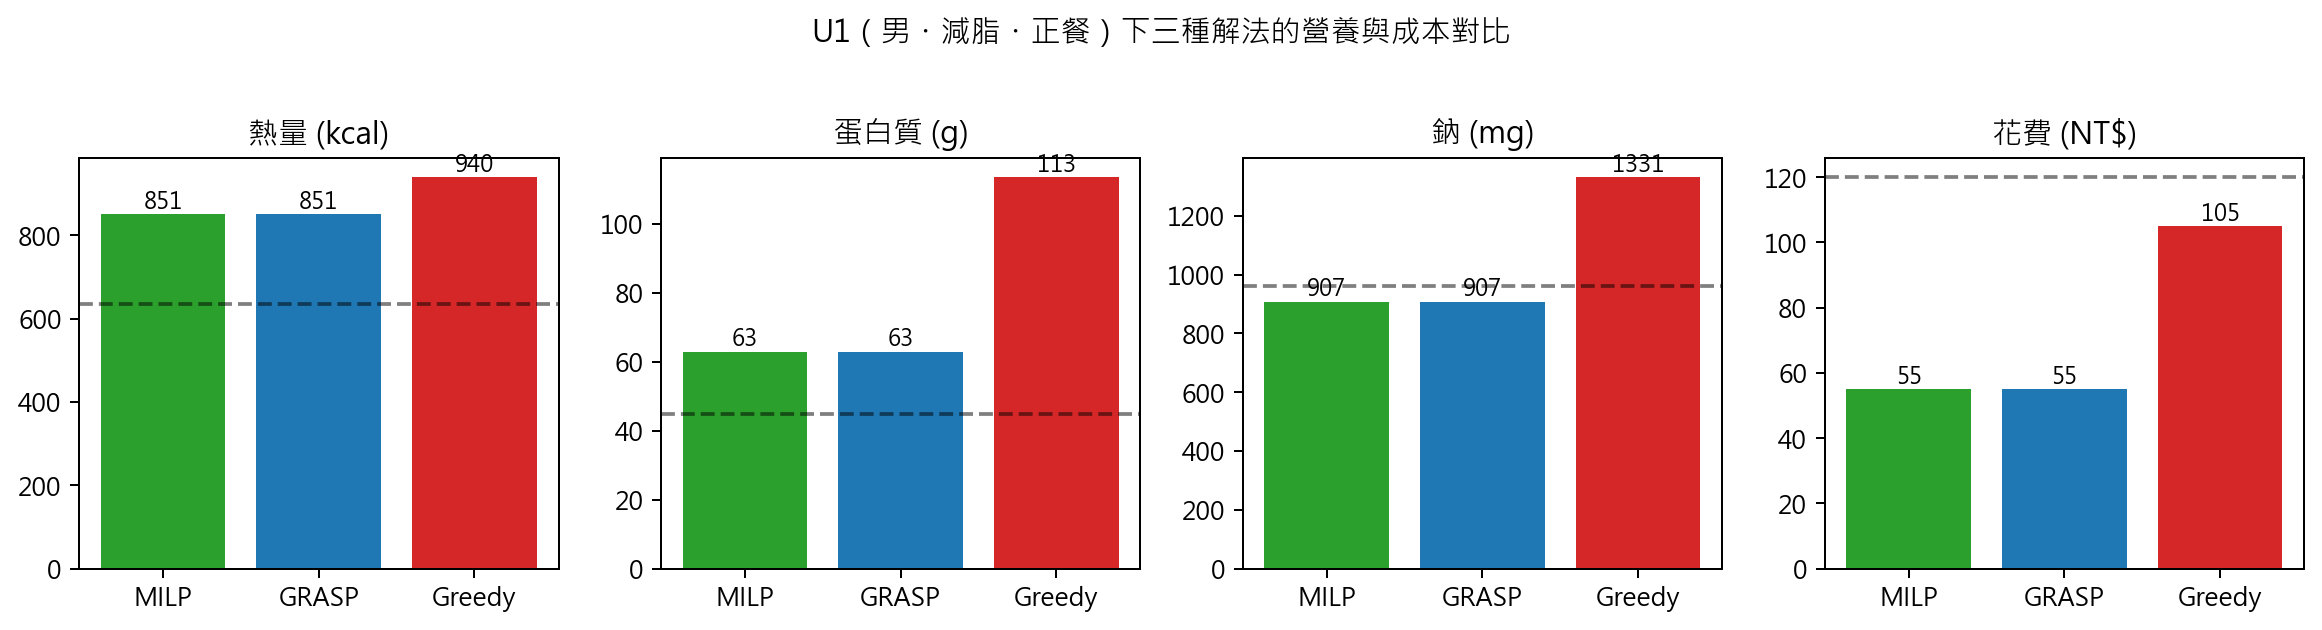
\includegraphics[width=0.95\textwidth]{../results/figs/fig_real_breakdown.png}\\
\small
U1 男·減脂·正餐：MILP/GRASP 取\textbf{結構完整的一餐}（主餐+配菜+飲料+甜點，NT\$110，全達標）；\\
Greedy 缺主餐、鈉破 $1.5\times$ 硬上限 $\Rightarrow$ \alert{hard-infeasible}。
\end{frame}

\begin{frame}{18 個真實例題 — 可行性與最佳化差距}
\begin{columns}[c]
\column{0.5\textwidth}
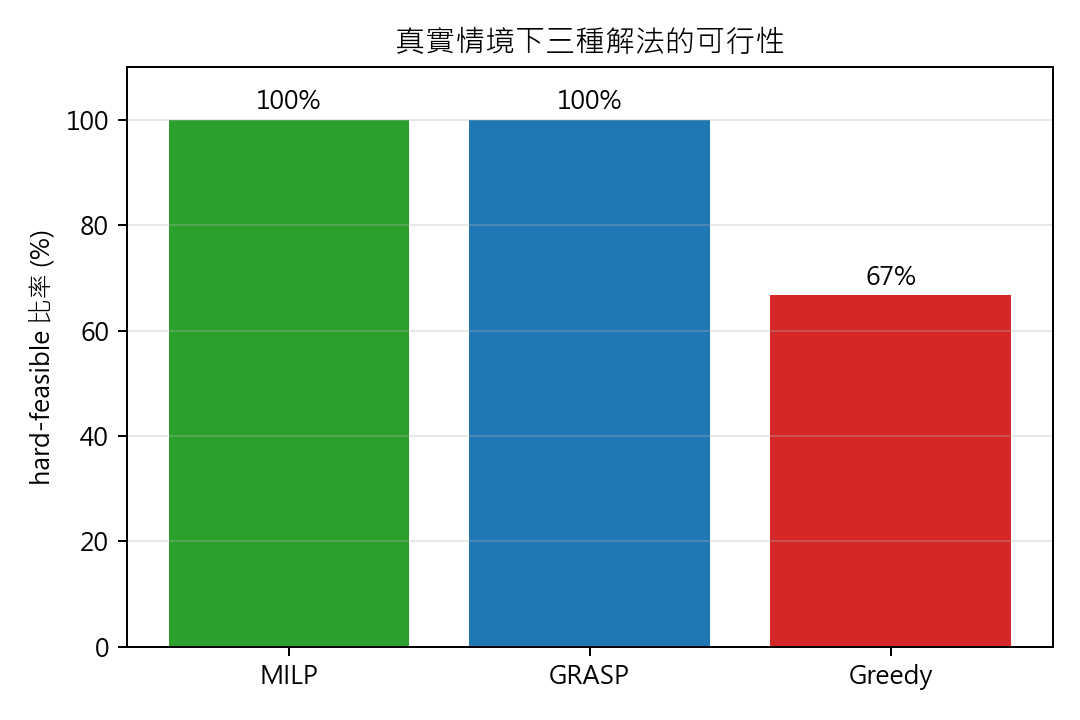
\includegraphics[width=\textwidth]{../results/figs/fig_feasibility.png}
\column{0.5\textwidth}
\textbf{結果摘要}
\begin{itemize}
  \item MILP：100\% 全域最佳解
  \item \alert{GRASP-LS：100\% hard-feasible，平均 gap 7.1\%}（12/18 為 0\%）
  \item \alert{Greedy：0\% feasible}（結構 + 鈉硬上限下全面失效）
  \item 非零 gap 全出現於正餐情境（結構限制使可行組合變窄）
\end{itemize}
\end{columns}
\end{frame}

\begin{frame}{互動式網頁應用（Flask）}
\centering
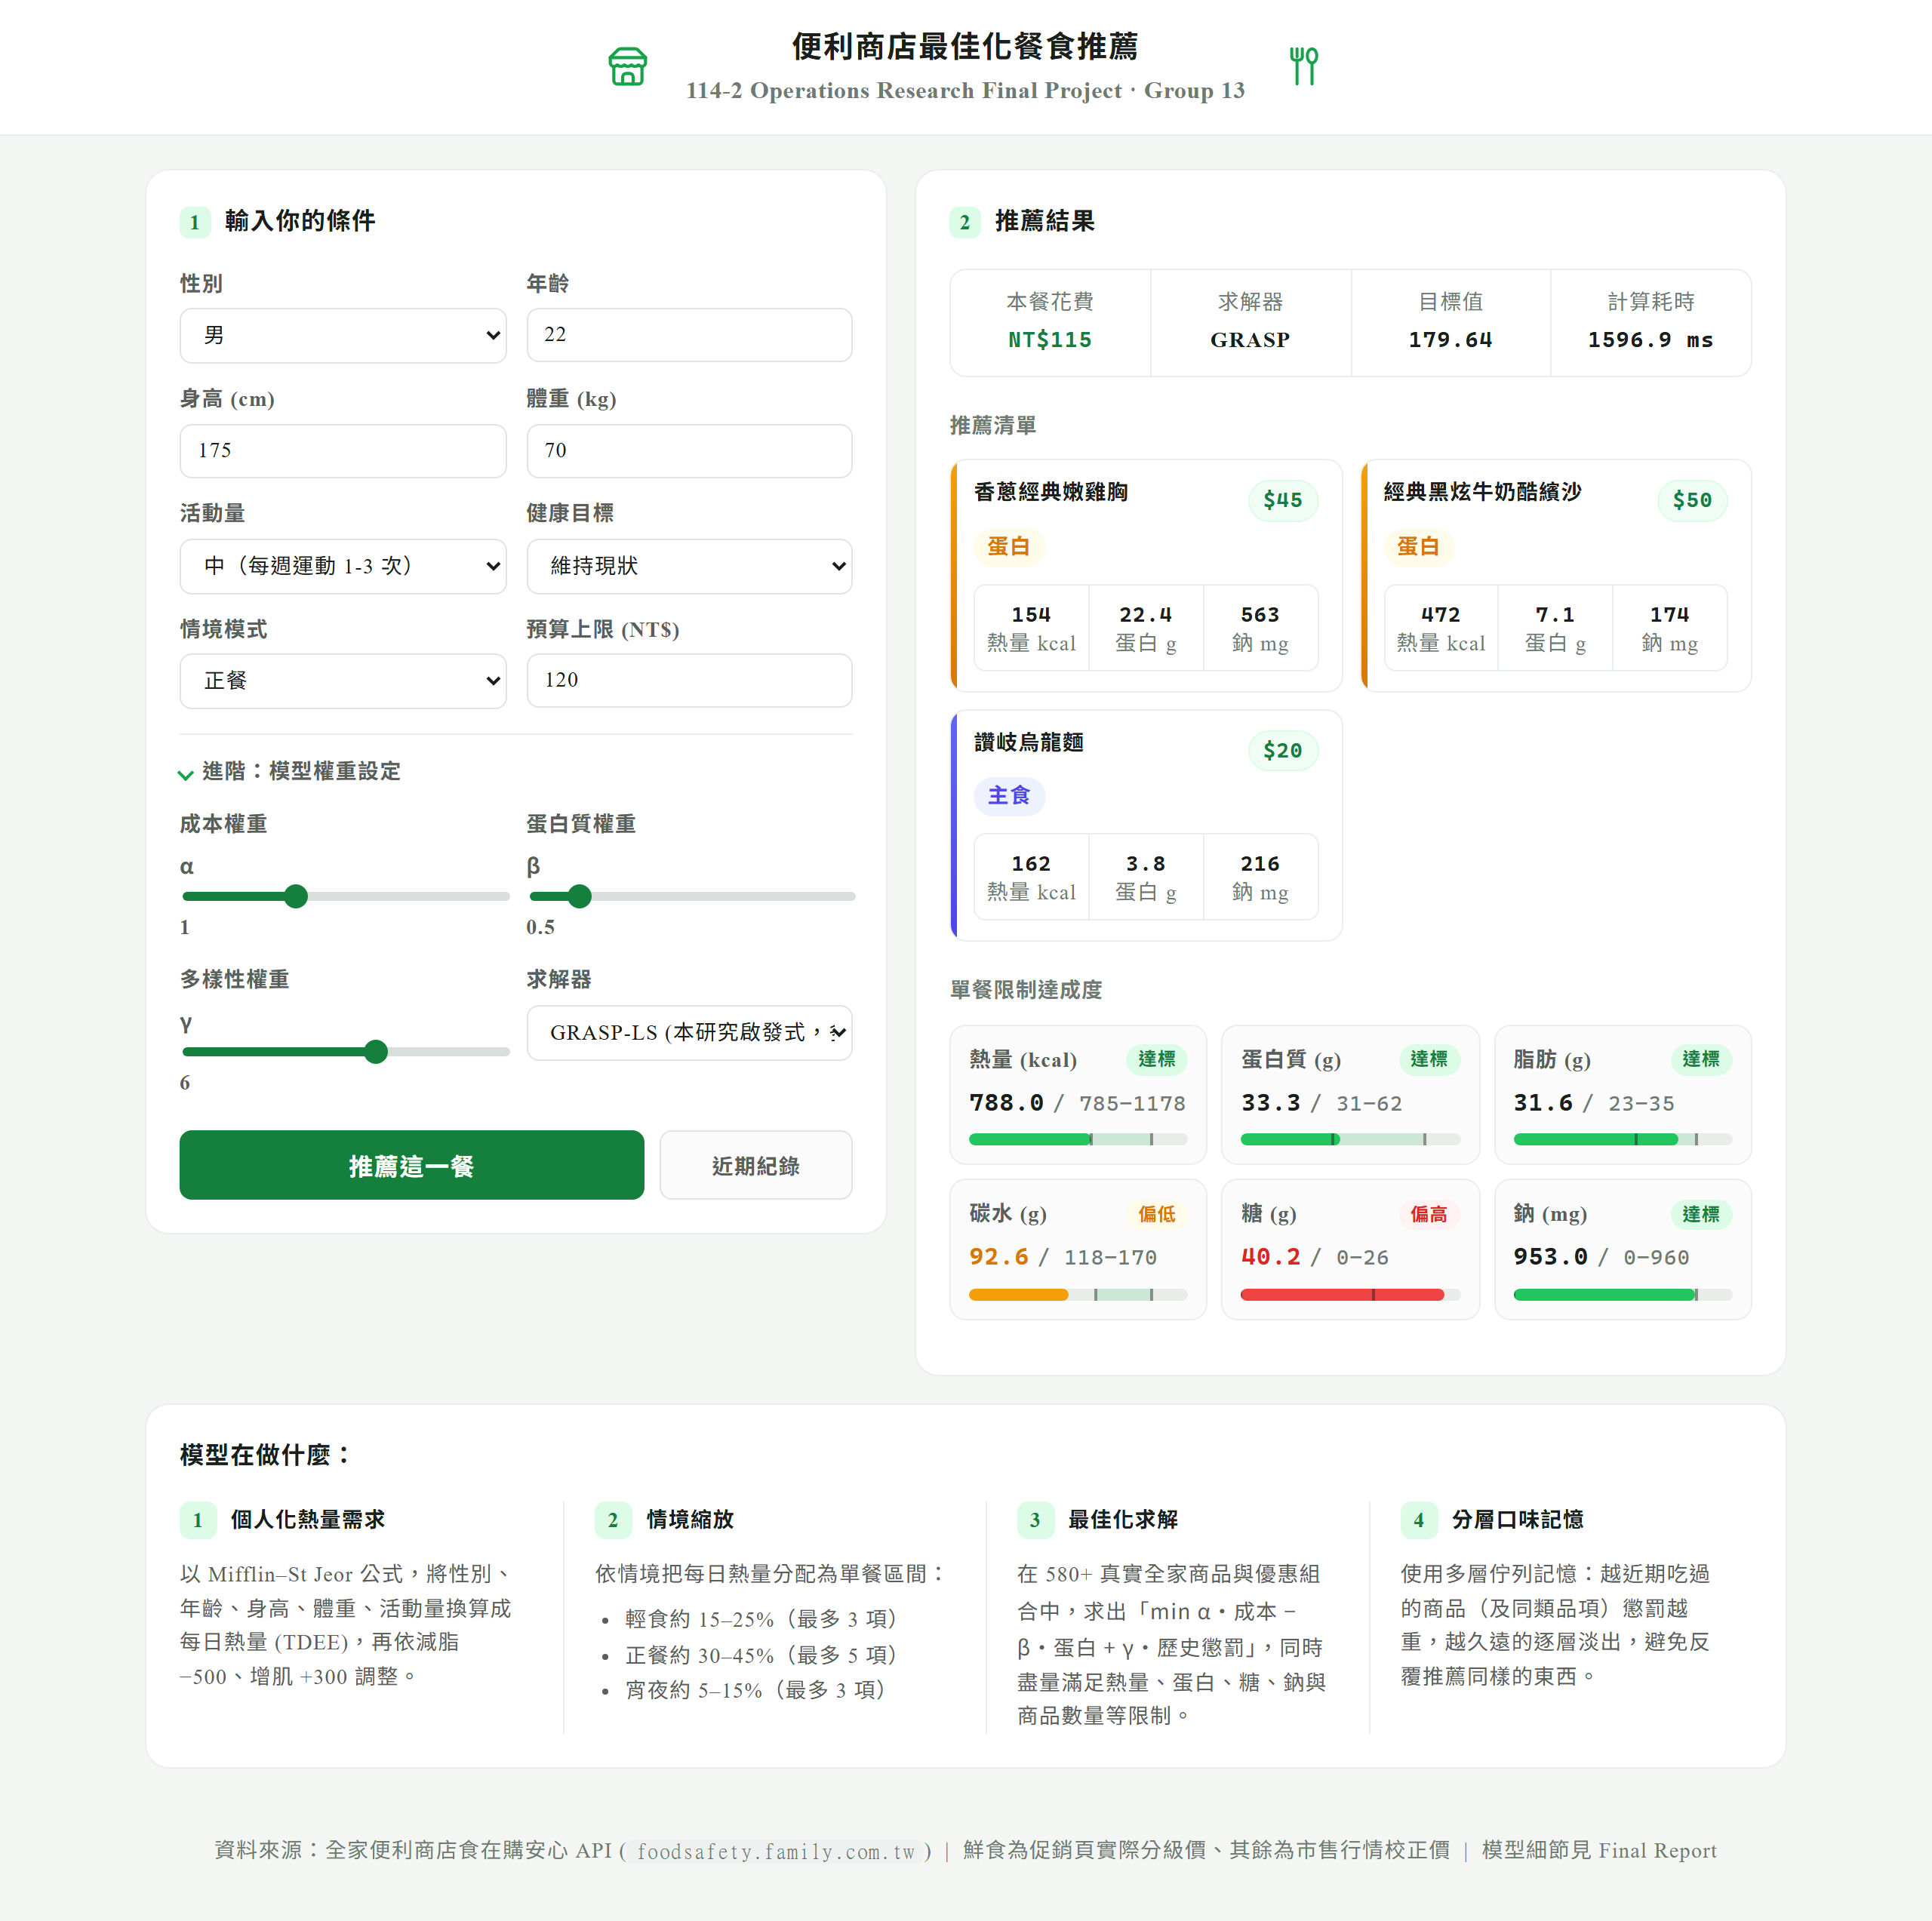
\includegraphics[width=0.88\textwidth]{../results/figs/webapp_result.png}\\
\small 使用者輸入 → Mifflin-St Jeor 換算 → GRASP/MILP 求解 → 即時推薦清單。\\
分層「口味記憶」(剛吃過/前幾餐/久未推) · slider 調整 $\alpha,\beta,\gamma$ · 跑在 488 項真實商品上。
\end{frame}

\begin{frame}{隨機例題：scalability 與 gap}
\begin{columns}[c]
\column{0.5\textwidth}
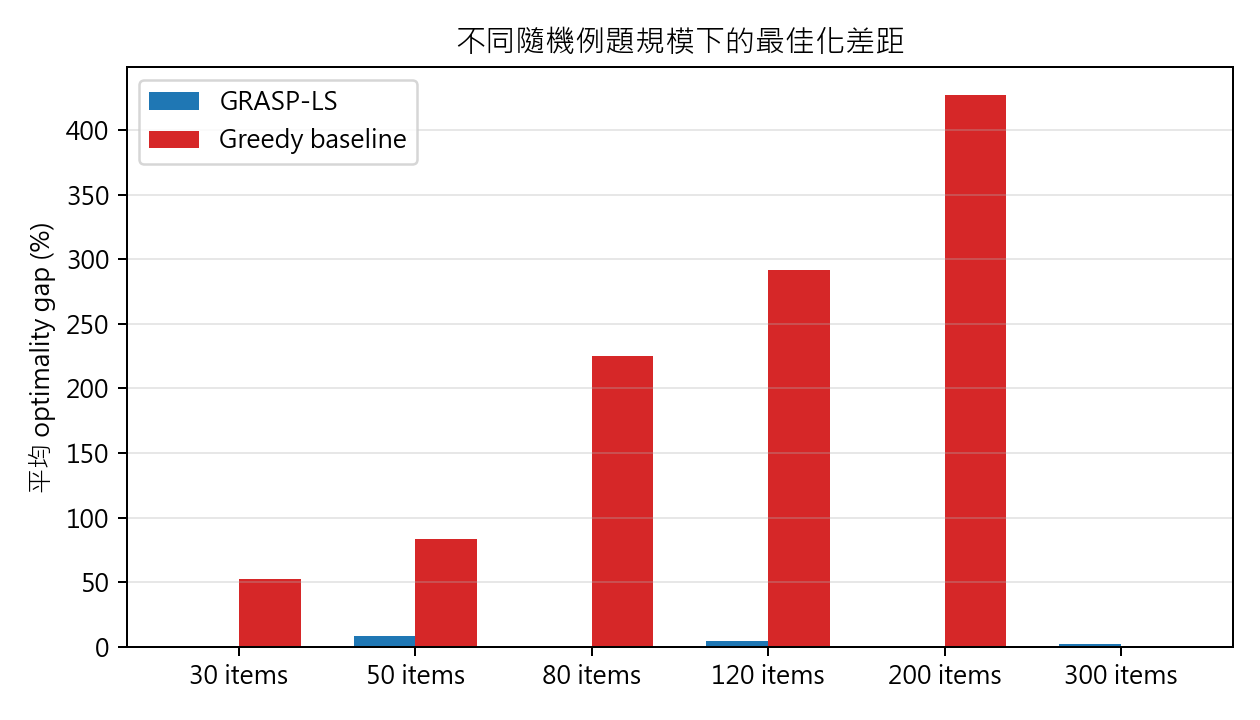
\includegraphics[width=\textwidth]{../results/figs/fig_gap_by_size.png}
\column{0.5\textwidth}
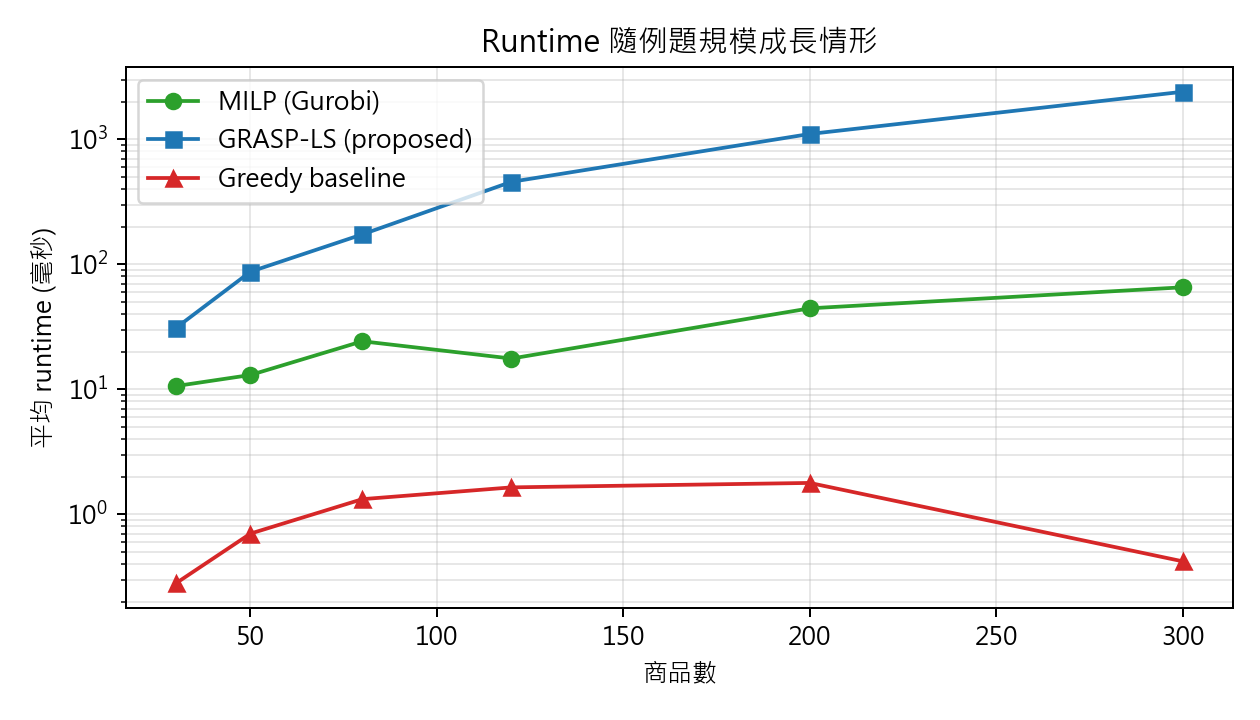
\includegraphics[width=\textwidth]{../results/figs/fig_runtime.png}
\end{columns}
\medskip\small
\begin{itemize}
  \item \alert{Greedy 多數規模 0\% 可行}（結構 + 鈉硬上限）
  \item \textbf{GRASP-LS} 平均 gap 4.9\%、feasible 93\%（28/30）
  \item MILP 227ms / GRASP 4.2s / Greedy <7ms @ $|I|=300$
\end{itemize}
\end{frame}

\begin{frame}{敏感度分析：權重 $\beta$ 與 $\gamma$}
\begin{columns}[c]
\column{0.5\textwidth}
\textbf{$\beta$：成本-蛋白質權衡}\\
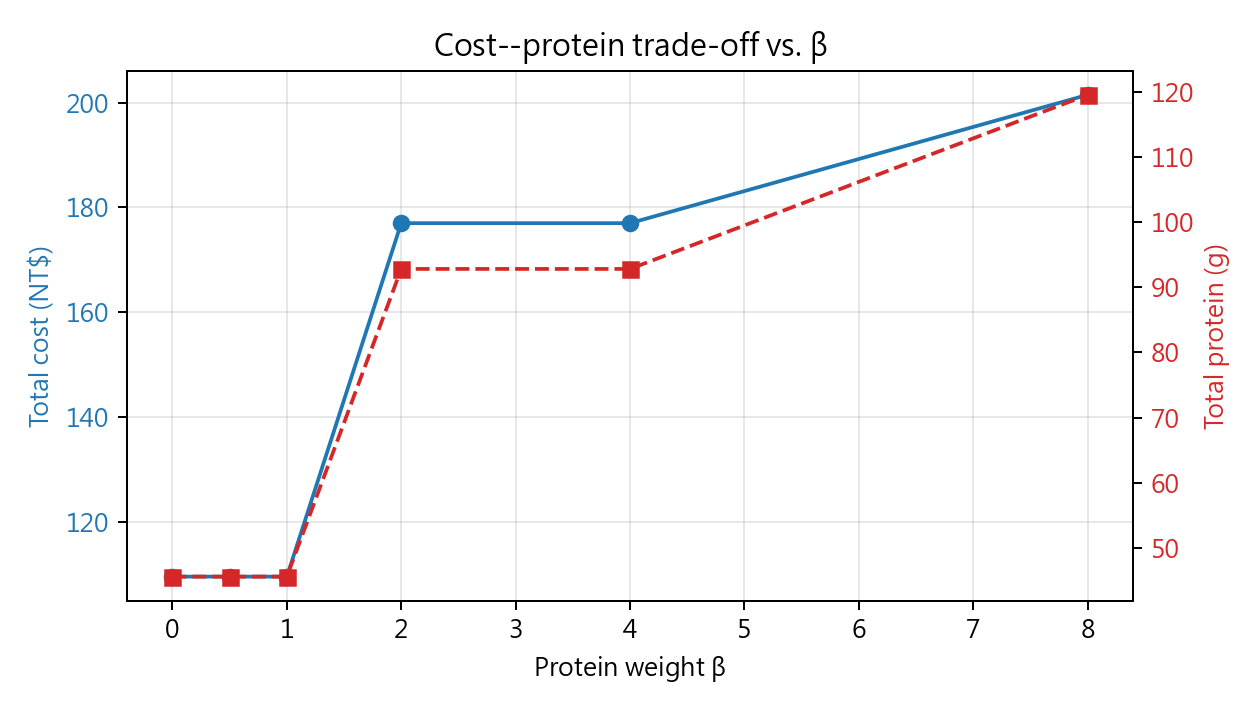
\includegraphics[width=\textwidth]{../results/figs/fig_beta_tradeoff.png}\\
\small{$\beta\le1$：NT\$109／45.6g；$\beta\ge2$ 階梯跳到 92.8g；$\beta=8$：119.5g／NT\$201}
\column{0.5\textwidth}
\textbf{$\gamma$：分層記憶／多樣性}\\
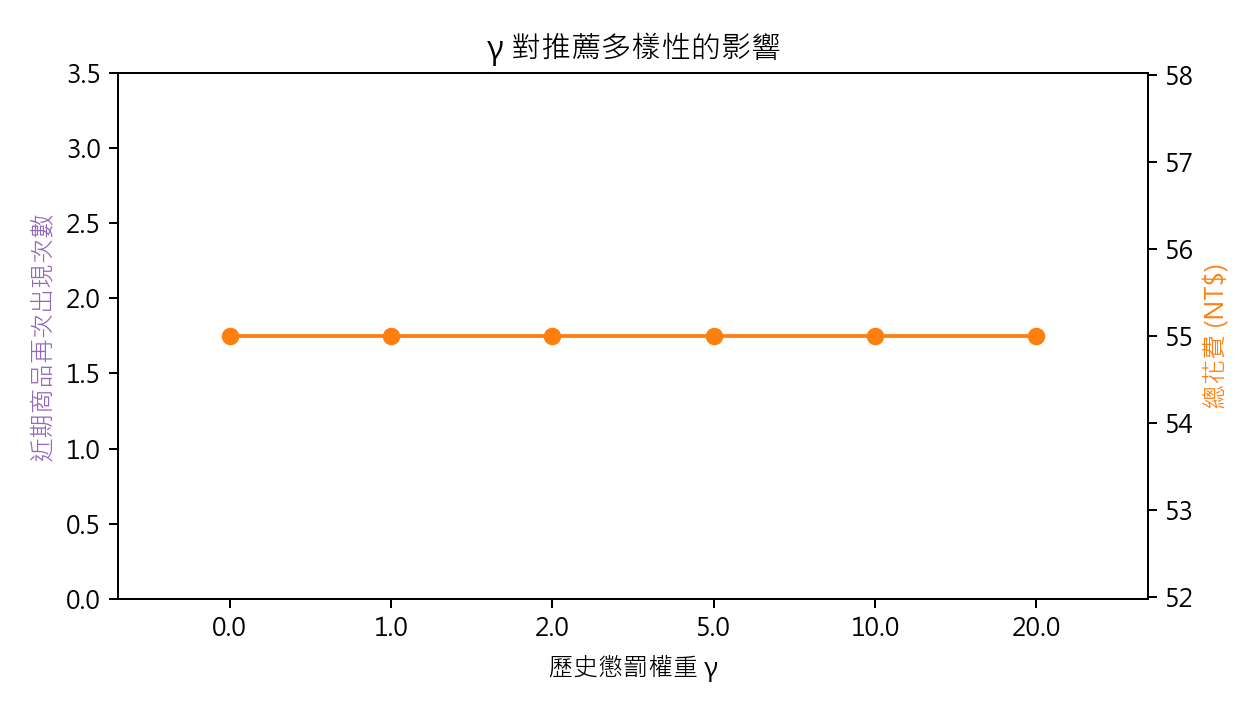
\includegraphics[width=\textwidth]{../results/figs/fig_gamma_diversity.png}\\
\small{注入 $\gamma=0$ 最優解為歷史，$\gamma\ge1$ 重複歸零，花費反降 NT\$109.5$\to$103}
\end{columns}
\end{frame}

\begin{frame}{多樣性的代價}
\begin{columns}[c]
\column{0.52\textwidth}
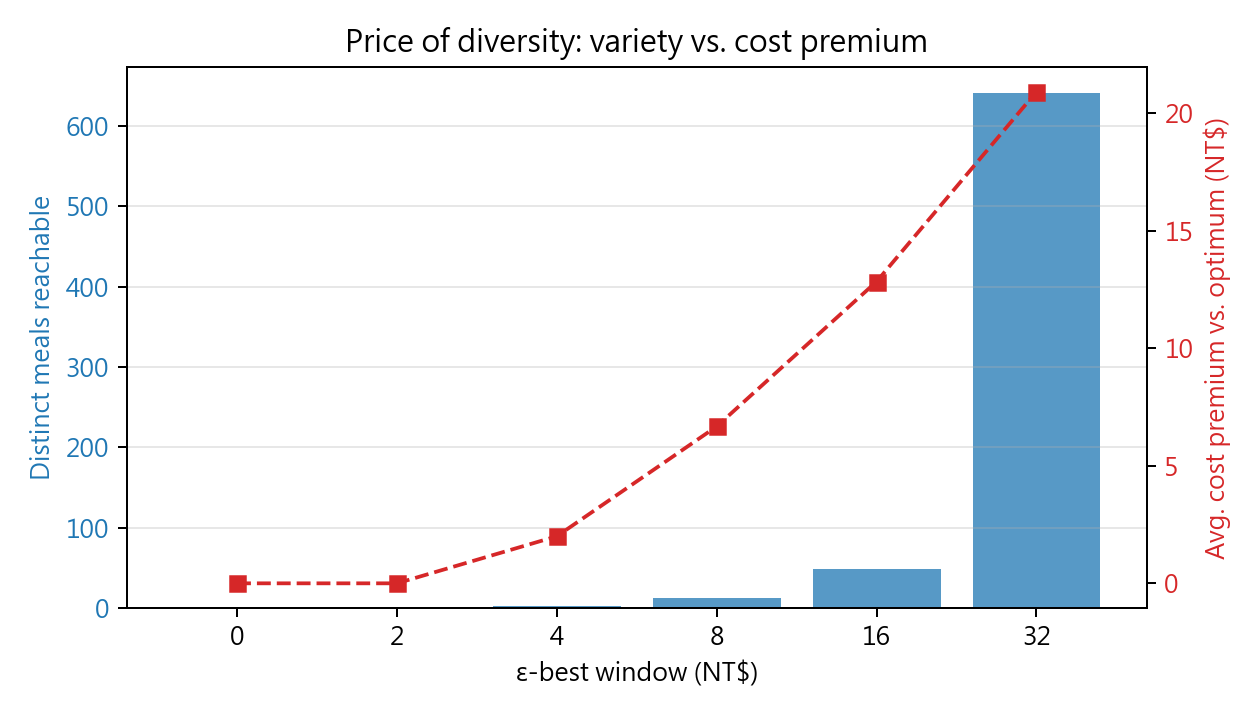
\includegraphics[width=\textwidth]{../results/figs/fig_price_of_diversity.png}
\column{0.48\textwidth}
\textbf{以 Gurobi 解池窮舉 $\epsilon$-最佳解集合}
\[ \mathcal{S}_\epsilon=\{s: z(s)\le z^*+\epsilon\} \]
\begin{itemize}
  \item $\epsilon=0$：僅 \textbf{1} 種最佳餐
  \item $\epsilon=8$：\textbf{12} 種達標餐，平均僅多 NT\$6.7
  \item $\epsilon=16$：48 種；$\epsilon=32$：\textbf{641} 種
\end{itemize}
\alert{在最佳解附近，多樣性極為廉價}——部署即以 $\epsilon=8$ 取樣 + 分層記憶長期去重。
\end{columns}
\end{frame}

% ============================================================
\section{Conclusion}
\begin{frame}{結論與洞察}
\textbf{學術貢獻}
\begin{itemize}
  \item 形式化為一含優惠組合、個人化營養、\textbf{餐型結構}與\textbf{分層多樣性懲罰}的 MILP
  \item GRASP-LS 啟發式：100\% feasible、平均 gap \textbf{7.1\%}／\textbf{4.9\%}、anytime
  \item 以 Gurobi 解池量化「\textbf{多樣性的代價}」；488 項真實商品 + Flask web app
\end{itemize}
\bigskip
\textbf{實務洞察}
\begin{itemize}
  \item \textbf{單一指標排序不能取代多限制最佳化}：Greedy 在新結構下 \alert{0\% 可行}
  \item \textbf{餐型結構 + 角色標記}讓推薦從「湊營養」變成「像一餐」
  \item \textbf{多樣性極廉}：容忍 NT\$8 即有 12 種達標餐；分層歷史懲罰甚至不漲價
  \item \textbf{$\beta$ 是個人化抓手}：使用者可以 slider 調節成本／蛋白質偏好
\end{itemize}
\end{frame}

\begin{frame}{未來工作}
\begin{itemize}
  \item \textbf{多日連續推薦：}將每日限制改為週期性限制；加入到貨／庫存波動。
  \item \textbf{OCR 商品標示：}店面實際拍照，自動更新資料表
  \item \textbf{線上學習：}使用者點擊／拒絕回饋更新 $h_i$ 與權重
  \item \textbf{多通路整合：}7-11 / Hi-Life / 全家併同決策；含時段限定品
  \item \textbf{鄰域擴充：}加入 2-2 swap、ejection chain 進一步縮小 GRASP 與 MILP 差距
\end{itemize}
\bigskip
\centering\Large
\textbf{Thank you! Questions?}
\end{frame}

\end{document}
